\section{Constructive Metaheuristics}

The constructive algorithms have strong limitations on many problems. What can be done, without abandoning the general scheme? \\

\textbf{Iterate the scheme} to generate many (potentially) \textbf{different solutions}:
\begin{itemize}
	\item the \textbf{efficiency decreases}: the computational times are summed
	\item the \textbf{effectiveness increases}: the best solution is returned
\end{itemize}

The trade-off must be carefully tuned.\\

The iterated scheme can apply
\begin{itemize}
	\item \textbf{multi-start}, that is \textbf{different algorithm} at \textbf{each iteration} $l = 1,\, ... \, , \ell$ (this requires to define multiple $\mathcal{F}_{A_l}$ and $\varphi_{A_l}$)
\end{itemize}

but it is more flexible to apply \textbf{metaheuristics}, that exploit
\begin{itemize}
	\item \textbf{randomization} (operations based on a random seed), as in the case of semigreedy algorithms, \textit{GRASP} and \textit{Ant System} (partly, \textit{ART})
	
	\item \textbf{memory} (operations based on the solutions of previous iterations), as in the case of \textit{ART}, cost perturbation and \textit{Ant System}
\end{itemize}

\paragraph{Termination condition:} The iterated scheme can ideally proceed for an infinite time.\\
In pratice, one uses termination conditions that can be "absolute"

\begin{enumerate}
	\item a given \textbf{total number of iterations} of the basic scheme
	
	\item a given \textbf{total execution time}
	
	\item a given \textbf{target value of the objective}
\end{enumerate}

or "relative" to the profile of $f^\ast$
\begin{enumerate}
	\item a given \textbf{number of iterations} of the basic scheme \textbf{without improving} $f^\ast$
	
	\item a given \textbf{execution time without improving} $f^\ast$
	
	\item a given \textbf{minimum ratio between the improvement} of $f^\ast$ and the \textbf{number of iterations} of the basic scheme \textbf{or the execution time} (e.g.: $f^\ast$ improves less than $1\%$ in the last $1000$ iterations)
\end{enumerate}

Fair comparisons require absolute conditions.

\newpage

\paragraph{Multi-start:} (or restart) is a classical, very simple and natural approach:
\begin{itemize}
	\item define \textbf{different search spaces} $F_{A^{[l]}}$ and \textbf{selection criteria} $\varphi_{A^{[l]}} (i, x)$
	
	\item \textbf{apply each} resulting \textbf{algorithm} $A^{[l]}$ to obtain the respective solution $x^{[l]}$
	
	\item \textbf{return the best solution} $x = \arg \min_{l = 1, \, ... \, , \ell} f(x^{[l]})$
\end{itemize}

A \textbf{typical case} is to \textbf{tune} $\varphi_A (i, x)$ with numerical parameters $\mu$.\\

The \textbf{construction graph can model this situation} by
\begin{itemize}
	\item including \textbf{all nodes and arcs admitted by at least one algorithm} $A^{[l]}$:
	$$ \mathcal{F}_A = \bigcup_{l=1}^\ell \mathcal{F}_{A^{[l]}} $$
	
	\item setting \textbf{arc weights depending on} $l: \varphi_A (i, x, l) = \varphi_{A^{[l]}} (i, x)$
	
	\item setting an \textbf{infinite arc weight} for the \textbf{arcs} that are \textbf{forbidden in a specific algorithm} $A^{[l]}:\varphi_A (i, x, l) = + \infty$
\end{itemize}

Essentially, this means defining and running different heuristics one after the other and returning the best solution found.\\

Example: a family of heuristics for the TSP can be obtained setting:
\begin{itemize}
	\item \textbf{insertion criteria:}
	$$ i^\ast_k = \arg \min_{i \in \{1, \, ... \, , |x|\}} \gamma_{i,k} = \mu_1 (c_{s_i, k} + c_{k, s_{i+1}}) - (1 - \mu_1)c_{s_i, s_{i+1}} $$
	where $\mu_1 \in [0; 1]$ tunes the relative strength of the
	\begin{itemize}
		\item increase in cost due to the added node $k$
		\item decrease in cost due to the removed edge $(s_i , s_{i+1})$
	\end{itemize}
	
	\item \textbf{selection criteria:}
	$$ k^\ast \arg \min_{k \in N \setminus N_x} \varphi_A (k,x) = \mu_2 \gamma_{i_k^\ast, k} + \mu_3 d(x,k) + (1 - \mu_2 - \mu_3) (-d (x,k)) $$
	where $\mu_2, \mu_3 \in [0; 1]$ tune the relative strength (and sign) of the
	\begin{itemize}
		\item increase in cost due to the added node $k$
		\item distance of the added node $k$ from the current circuit $x$
	\end{itemize}
\end{itemize}

This yields CI for $\mu = (1/2, 1, 0)$, NI for $\mu = (1/2, 0, 1)$, FI for $\mu = (1/2, 0, 0)$.\\

\newpage

\subsection{Constructive metaheuristics}
The main constructive metaheuristics are
\begin{enumerate}
	\item \textbf{Adaptive Research Technique (ART) or Tabu Greedy:} forbid some moves based on the solutions of the previous iterations
	$$ \min_{i \in \Delta_{A^{[l]}}^+ (x) } \varphi_A (i, x) $$
	$$ \text{with } \Delta_{A^{[l]}}^+ (x) = \left\{ i \in B \setminus x: \, x \cup \left\{i\right\} \in \mathcal{F}^{[l]} \left(x_A^{[1]}, \, ... \, , x_A^{[l-1]}\right) \subseteq \mathcal{F} \right\}$$
	This is much less popular than the other two.\\
	A greedy algorithm with some "taboo", dome forbidden choices; same selection criteria but restricted search space based on previous solutions.\\
	
	\item \textbf{Semigreedy and GRASP:} use a randomized selection criteria
	$$ \min_{i: \, x \cup \left\{i\right\} \in \mathcal{F}} \varphi_A^{[l]} \left(i, x, \omega^{[l]}\right) $$
	The selection criteria has a random element, the selection will be partly stochastic. The search space is fixed.\\
	
	\item \textbf{Ant System (AS):} use a randomized selection criteria depending on the solutions of the previous iterations
	$$ \min_{i: \, x \cup \left\{i\right\} \in \mathcal{F}} \varphi_A^{[l]} \left(i, x, \omega^{[l]}, x_A^{[1]}, \, ... \, , x_A^{[l-1]}\right) $$
	Apply both a random selection and dependence on previous solutions.\\
\end{enumerate}

New information on the arcs of the construction graph guides the search.\\
The ART uses memory, the GRASP randomization, the AS both.\\

\newpage

\subsection{Adaptive Research Technique ART}
It was proposed by Patterson et al. (1998) for the CMSTP.\\

When \textbf{deceivingly good elements} are included in the \textbf{first steps} the \textbf{final solution can be quite bad}.\\

Aiming to avoid that
\begin{itemize}
	\item The roll-out approach makes a look-ahead on each possible element (but a single step can be insufficient to identify the misleading ones).\\
	
	\item The \textbf{ART forbids some elements} to \textbf{drive subset} $x$ \textbf{on the right path} in the search space (how to identify the misleading elements?).\\
\end{itemize}

Forbidding elements of the previous solution guarantees to obtain different solutions.\\

The \textbf{prohibitions are temporary}, with an expiration time of $L$ iterations; otherwise, building feasible solutions would soon become impossible.\\

\newpage

\paragraph{How does it work?} Define a basic constructive heuristic $A$.\\

Let $T_i$ be the \textbf{starting iteration of the prohibition} for each element $i \in B$ and $x^\ast$ be the best solution found. Essentially a vector that keeps track of when the prohibition starts.\\

Set $T_i = −\infty$ for all $i \in B$ to indicate that \textbf{no element} is \textbf{forbidden}.\\

At \textbf{each iteration} $l \in \{1, \, ... \, , \ell \}$
\begin{enumerate}
	\item Apply heuristic $A$ \textbf{forbidding all elements} $i$ \textbf{such that} $l \leq T_i + L$ (the current iteration must be less than the value at which the prohibition for that element started $+$ the expiration time $L$, thus all prohibitions older than $L$ iterations automatically expire); let $x^{[l]}$ be the \textbf{resulting solution}.\\
	
	\item If $x^{[l]}$ is better than $x^\ast$, set $x^\ast := x^{[l]}$ and save $T_i - l$ (to know which elements in the solution where forbidden and for how much time) for all $i \in B$.\\
	
	\item \textbf{Decide} which \textbf{elements to forbid} and set $T_i = l$ for them: each element is forbidden with probability $\pi$ (any better ideas?).\\
	
	\item Make minor tweaks to $L, \pi$ or $T_i$.\\
\end{enumerate}

At the end, \textbf{return} $x^\ast$ (best solution found).\\

\newpage

\paragraph{Example:} ART for the SCP 
$$
c \;\;\;\;
\begin{array}{| c c c c c |}
	\hline
	25 & 6 & 8 & 24 & 12 \\
	\hline
\end{array}
$$

$$
A \;\;\;\;
\begin{array}{| c c c c c |}
	\hline
	1 & 1 & 0 & 0 & 0 \\
	1 & 1 & 0 & 0 & 0 \\
	1 & 1 & 1 & 0 & 0 \\
	1 & 0 & 1 & 1 & 0 \\
	1 & 0 & 0 & 1 & 0 \\
	1 & 0 & 0 & 0 & 1 \\
	\hline
\end{array}
$$
Let $L = 2$, $\pi = 0.15$, pseudo-random numbers $0.1, 0.9, 0.4, 0.5, 0.1, 0.2, \, ...$
\begin{enumerate}
	\item the basic heuristic finds solution $x^{[1]} = \{2, 3, 5, 4\}$ of cost $f \left(x^{[1]}\right) = 50$; forbid column $2$ (because $0.1 \leq \pi < 0.9$, $0.4$ and $0.5$)
	
	\item the basic heuristic finds solution $x^{[2]} = \{3, 1\}$ ($2$ is forbidden) of cost $f \left(x^{[2]}\right) = 33$; forbid column $3$ (because $0.1 \leq \pi < 0.2$)
	
	\item the basic heuristic finds solution $x^{[3]} = \{1\}$ ($3$ and $2$ are forbidden) of cost $f = \left(x^{[3]}\right) = 25$, that is optimal
	
	\item ...
\end{enumerate}
An unlucky sequence could forbid column 1 at step 2.\\

\newpage

\subsubsection{Parameter tuning}
The ART has \textbf{three basic parameters}
\begin{itemize}
	\item the \textbf{total number of iterations} $\ell$ (tuned mainly by the available time)
	\item the \textbf{length} $L$ \textbf{of the prohibition}
	\item the \textbf{probability} $\pi$ \textbf{of the prohibition}
\end{itemize}

How to assign effective values to the parameters? \\

The \textbf{experimental comparison} of different values is necessary but complex
\begin{enumerate}
	\item it requires \textbf{long experimental campaigns}, because the number of configurations grows combinatorially with
	\begin{itemize}
		\item the number of parameters
		\item the number of tested values for each parameter
	\end{itemize}
	(the more sensitive the result, the more values must be tested)\\
	
	\item it \textbf{risks overfitting}, that is labeling as absolutely good values which are good only on the benchmark instances considered \\
\end{enumerate}

The excess of parameters is an undesirable aspect, and often reveals an insufficient study of the problem and of the algorithm.\\

\newpage

\subsubsection{Diversification and intensification}

\textbf{Diversification} aims to obtain different solutions at every iteration. The ART achieves it by forbidding elements of the previous solutions.\\
An excessive diversification can hinder the discovery of the optimum.\\

\textbf{Intensification} aims to focus the search on the more promising subsets.\\

Diversification and intensification play complementary roles.\\

Their relative strength can be tuned through the parameters based on
\begin{itemize}
	\item \textbf{problem data:} assign
	\begin{itemize}
		\item a \textbf{smaller probability} $\pi_i$ to be forbidden (forbidding a few elements)
		
		\item a \textbf{shorter expiration time} $L_i$ of the prohibition (forbidding for a short time)
	\end{itemize}
	\textbf{to promising elements} (e.g., cheaper ones). This can lead to intensification on promising solutions. \\
	
	\item \textbf{memory:}
	\begin{itemize}
		\item assign a \textbf{smaller} $\pi_i$ \textbf{or} $L_i$ ($i$ is never forbidden when $\pi_i = 0$ or $L_i = 0$) \textbf{to promising elements} (e.g., appearing in the best known solutions)
		
		\item \textbf{periodically restart the algorithm} with the $T_i - l$ values associated with the best known solution, instead of $T_i = - \infty$
	\end{itemize}
	This is trying to learn which parameters are "good" through past solutions.\\
\end{itemize}

\newpage

\subsection{Semi-greedy heuristics}
A \textbf{nonexact constructive algorithm} has \textbf{at least one step} $t$ which \textbf{builds a subset} $x^{(t)}$ \textbf{not included in any optimal solution} (since it's not the best, at one step it takes the wrong choice).\\

Since the element selected is the \textbf{best according to the selection criteria}
$$ i^\ast = \arg \min_{i \in \Delta_A^+ (x)} \varphi_A (i, x)$$
necessarily $\varphi_A (i, x)$ \textbf{is incorrect}, but probably \textbf{not completely wrong}.\\

The \textbf{semi-greedy algorithm} (Hart and Shogan, 1987) assumes that \textbf{elements that lead to the optimum are very good for} $\varphi_A (i, x)$, even if not strictly the best.\\

How to know which one?\\

If it is not possible to refine $\varphi_A (i, x)$
\begin{itemize}
	\item Define a \textbf{suitable probability distribution on} $\Delta_A^+ (x)$ \textbf{favoring} the \textbf{elements} with the \textbf{best values} of $\varphi_A (i, x)$.\\
	
	\item \textbf{Select} $i^\ast (\omega)$ \textbf{according to the distribution function}.\\
\end{itemize}

\newpage

Since the set of alternative choices is finite, this means to \textbf{assign}
\begin{itemize}
	\item \textbf{probability} $\pi_A (i, x)$ \textbf{to arc} $(x, x \cup \{i\})$ \textbf{of the construction graph} (with a sum equal to $1$ for the outgoing arcs of each node, total probability)
	$$ \sum_{i \in \Delta_A^+ (x)} \pi_A (i,x) = 1 \text{ for all } x \in \mathcal{F}_A : \, \Delta_A^+ (x) \neq \emptyset $$
	I have to get out of a node, each arc has a certain probability.\\
	
	\item \textbf{higher probabilities to the better elements} for the selection criteria
	$$ \varphi_A (i,x) \leq \varphi_A (j,x) \Leftrightarrow \pi_A (i,x) \geq \pi_A (j,x) $$
	for each $i, j \in \Delta_A^+ (x)$, $x \in \mathcal{F}_A$.\\
	If the selection criteria is less, the probability must be more (because it means that it could be a better path).\\
\end{itemize}

This heuristic approach has important properties
\begin{itemize}
	\item It can \textbf{reach an optimal solution} if there is a \textbf{path from} $\emptyset$ \textbf{to} $X^\ast$ (this is a basic condition).\\
	
	\item It can be \textbf{reapplied several times obtaining different solutions} and the probability to reach the optimum grows gradually (each iteration decreases the probability of missing an optimal path).\\
\end{itemize}

\newpage

\subsubsection{Convergence to the optimum}
The probability of
\begin{itemize}
	\item \textbf{following a path} $\gamma$ is the \textbf{product of the probabilities on the arcs}
	$$ \prod_{y, y \cup \left\{i\right\} \in \gamma} \pi_A (i, y) $$
	Each path is the product of every one of its arcs.\\
	
	\item \textbf{obtaining a solution} $x$ is the \textbf{sum of those of the paths} $\Gamma_x$ \textbf{reaching} $x$
	$$ \sum_{\gamma \in \Gamma_x} \;\; \prod_{y, y \cup \left\{i\right\} \in \gamma} \pi_A (i,y) $$
	The probability of a solution is the sum of the probability of all its possible paths.\\
\end{itemize}

This implies that the \textbf{probability to reach the optimum}:
\begin{enumerate}
	\item \textbf{Is nonzero} if and only \textbf{if there exists a path of nonzero probability} from $\emptyset$ to $X^\ast$.\\
	
	\item \textbf{Increases as} $\ell \rightarrow + \infty$ (the probability of not reaching it decreases gradually)
\end{enumerate}

It tends to $1$ for probabilistically approximately complete algorithms.\\

\newpage

In this context, a \textbf{random walk} is a constructive metaheuristic in which \textbf{all the arcs going out of the same node have equal probability}
\begin{itemize}
	\item it \textbf{finds a path to the optimum with probability 1} (if one exists)
	
	\item the \textbf{time required can be extremely long}. The exhaustive algorithm is exact and requires finite time
\end{itemize}

\nn

A \textbf{deterministic} constructive heuristic sets \textbf{all probabilities to zero} except for those on the \textbf{arcs of a single path}
\begin{itemize}
	\item it \textbf{finds the optimum only if it enjoys specific properties}
	\item it \textbf{finds the optimum in a single run}
\end{itemize} 
You just have the minimum selection criteria, which is chosen deterministically.\\


\textbf{Randomized} heuristics that \textbf{favor promising arcs and penalize the others}
\begin{itemize}
	\item \textbf{accelerate} the \textbf{average convergence time}
	\item \textbf{decrease} the \textbf{guarantee of convergence} in the worst case
\end{itemize}

There is a \textbf{trade-off between expected and worst result}.\\

Arcs with \textbf{zero probability} can \textbf{block the path to the optimum}.\\
Arcs with \textbf{probability converging to zero reduce the probability of finding it}.\\

\newpage

\subsection{GRASP and Semi-greedy}
GRASP, that is \textbf{Greedy randomized Adaptive Search Procedure} (Feo and Resende, 1989) is a more sophisticated variant of the semi-greedy heuristic
\begin{itemize}
	\item \textbf{Greedy} indicates that it uses a constructive basic heuristic
	
	\item \textbf{Randomized} indicates that the basic heuristic makes random steps
	
	\item \textbf{Adaptive} indicates that the heuristic uses an adaptive selection criteria $\varphi_A (i, x)$, depending also on $x$ (not strictly necessary)
	
	\item \textbf{Search} indicates that it alternates the constructive heuristic and an exchange heuristic (differently from the semi-greedy approach)
\end{itemize}

The use of auxiliary exchange heuristics allows strongly better results.\\

\paragraph{What probability function?} Several functions $\pi_A (i, x)$ are monotonous with respect to $\varphi_A (i, x)$
$$ \varphi_A (i,x) \leq \varphi_A (j,x) \Leftrightarrow \pi_A (i,x) \geq \pi_A (j,x) $$
Better value of the selection criteria correspond to larger probabilities.

\begin{itemize}
	\item \textbf{uniform probability:} each arc going out of $x$ has the same $\pi_A (i, x)$; the algorithm performs a random path in $\mathcal{F}_A$ (random walk).\\
	
	\item \textbf{Heuristic-Biased Stochastic Sampling (HBSS):}
	\begin{itemize}
		\item sort the arcs going out of $x$ by nonincreasing (best first) values of $\varphi_A (i, x)$
		\item assign a decreasing probability according to the position in the order based on a simple scheme (linear, exponential, ecc...)
	\end{itemize}
	Assign a probability to each arc depending on its position in the "ranking list".\\
	
	\item \textbf{Restricted Candidate List (RCL):}
	\begin{itemize}
		\item sort the arcs going out of $x$ by nonincreasing values of $\varphi_A (i, x)$
		\item insert the best arcs in a list (How many?)
		\item assign uniform probability to the arcs of the list, zero to the others
	\end{itemize}
	It just takes a subset containing the best arcs.\\
\end{itemize}

The most common strategy is the RCL, even if the zero probability arcs potentially cancel the global convergence to the optimum.

\newpage

\subsubsection{Definition of the RCL}
Two main strategies are used to define the RCL
\begin{itemize}
	\item \textbf{Cardinality:} the RCL includes the \textbf{best} $\mu$ \textbf{elements of} $\Delta_A^+ (x)$, where $\mu \in \{1,\, ... \, , |\Delta_A^+(x)|\}$ is a parameter fixed by the user
	\begin{itemize}
		\item $\mu = 1$ yields the constructive basic heuristic (takes only the best)
		\item $\mu = |B|$ (i, e., $|\Delta_A^+ (x)|$ for each $x$) yields the random walk (takes all the choices)
	\end{itemize}
	You decide that you want to take $\mu$ elements (usually fixed), each node will have $\mu$ outgoing arcs.\\
	
	\item \textbf{Value:} the RCL includes \textbf{all} the \textbf{elements} of $\Delta_A^+ (x)$ whose \textbf{value is between} $\varphi_{min}$ \textbf{and} $(1 − \mu) \varphi_{min} + \mu \varphi_{max}$ (for minimization problems) where
	$$ \varphi_{min} (x) = \min_{i \in \Delta_A^+ (x)} \varphi_A (i,x) \;\;\;\;\; \varphi_{max} = \max_{i \in \Delta_A^+ (x)} \varphi_A (i,x) $$
	and $\mu \in [0; 1]$ is a parameter fixed by the user
	\begin{itemize}
		\item $\mu = 0$ yields the constructive basic heuristic (takes only the minimum)
		\item $\mu = 1$ yields the random walk (takes everything from minimum to maximum)
	\end{itemize}
	This takes all the solution in a certain "range of quality", determined by the parameter $\mu$ and the overall total quality range.\\
\end{itemize}

\newpage

\paragraph{Example:} GRASP for the SCP 
$$
c \;\;\;\;
\begin{array}{| c c c c c |}
	\hline
	25 & 6 & 8 & 24 & 12 \\
	\hline
\end{array}
$$

$$
A \;\;\;\;
\begin{array}{| c c c c c |}
	\hline
	1 & 1 & 0 & 0 & 0 \\
	1 & 1 & 0 & 0 & 0 \\
	1 & 1 & 1 & 0 & 0 \\
	1 & 0 & 1 & 1 & 0 \\
	1 & 0 & 0 & 1 & 0 \\
	1 & 0 & 0 & 0 & 1 \\
	\hline
\end{array}
$$

Let $\mu = 2$ and the pseudo-random sequence be: $0.6, 0.8, \, ...$
\begin{enumerate}
	\item Start with the empty subset: $x^{(0)} = \emptyset$.\\
	
	\item Build the RCL with columns $2 (\varphi_2 = 2)$ and $3 (\varphi_3 = 4)$; select column $3$ (because $0.6 > 1/2$).\\
	
	\item Build the RCL with columns $2 (\varphi_2 = 3)$ and $1 (\varphi_1 = 6.25)$; select column $1$ (because $0.8 > 1/2$).\\
	
	\item The solution obtained is $x = \{3, 1\}$ of cost $f (x) = 33$.\\
\end{enumerate}

With $\mu = 2$, the optimal solution cannot be obtained; while with $\mu = 3$ it can be (the first column is the third in respect to the first selection criteria).\\

The optimum can be found with $\mu = 2$ if a destructive phase is applied.\\

\newpage

\subsubsection{Reactive parameter tuning}

Once again there are \textbf{parameters to tune}:
\begin{itemize}
	\item the \textbf{number of iterations} $\ell$ (for each "generation")
	\item the \textbf{value} $\mu$ determining the \textbf{size of the RCL}
\end{itemize}

An idea to exploit memory is to \textbf{learn from the previous results} (reactive because it reacts to previous results)
\begin{enumerate}
	\item Select $m$ \textbf{configurations of parameters} $\mu_1,\, ... \, , \mu_m$ and set $\ell_r = \ell/m$ (divide the whole set of iteration in $m$ parts, one for each parameter).\\
	
	\item Run each configuration $\mu_r$ for $\ell_r$ iterations (same number for each, obtaining $\ell_r$ different solutions).\\
	
	\item \textbf{Evaluate} the \textbf{mean} $\overline{f} (\mu_r)$ of the \textbf{results obtained with} $\mu_r$ (results obtained in the iterations with a certain parameter).\\
	
	\item \textbf{Update the number of iterations} $\ell_r$ for each $\mu_r$ based on $\overline{f} (\mu_r)$
	$$ \ell_r = \frac{ \frac{ 1}{ \overline{f} (\mu_r) } } { \sum_{s=1}^m \frac{ 1 }{ \overline{f} (\mu_s) }} \ell \;\; \text{ for } r = 1, \, ... \, m $$
	\textbf{increasing it for the more effective configurations} (more iterations to good configurations, less to bad ones).\\
	The formula above makes a number $\in [0,1]$ (then multiplied by the number of iterations $\ell$) which is small for big values of $\overline{f} (\mu_r)$ and vice versa (minimization problem).\\
	
	\item \textbf{Repeat the whole process}, going back to point $2$, for $R$ times (total number of "generation").\\
	
\end{enumerate}
Other schemes use scores based on the number of best known results.\\

You set $m$ different parameters and you adjust the time dedicated to each based on their performance.\\

\newpage

\subsection{Cost perturbation methods}

Instead of forbidding/forcing some choices, or modifying their probability, it is possible to \textbf{modify the appeal of the available choices} (selection criteria).\\

Given a basic constructive heuristic $A$, at each step of iteration $l$
\begin{itemize}
	\item \textbf{tune the selection criteria} $\varphi_A (i, x)$ with a factor $\tau_A^{[l]} (i, x)$
	$$ \psi_A^{[l]} (i,x) = \frac{\varphi_A (i,x)}{\tau_A^{[l]} (i, x)} $$
	
	\item \textbf{update} $\tau_A^{[l]} (i, x)$ based on the previous solutions $x^{[1]}, \, ... \, , x^{[l−1]}$
\end{itemize}
The selection criteria is multiplied by a factor $\tau$ associated to the arcs ($(i,x)$ like the selection criteria) and can vary from iteration to iteration ($^{[l]}$)

The elements with a better $\varphi_A (i, x)$ tend to be favored, but $\tau_A^{[l]} (i, x)$ tunes this effect, promoting
\begin{itemize}
	\item \textbf{intensification} if $\tau_A^{[l]} (i, x)$ increases for the most frequent elements; this favors solutions similar to the previous ones (if the solutions are good)
	
	\item \textbf{diversification} if $\tau_A^{[l]} (i, x)$ decreases for the most frequent elements; this favors solutions different from the previous ones
\end{itemize}

\newpage

\subsection{Ant Colony Optimization}

It was devised by Dorigo, Maniezzo and Colorni in 1991 drawing inspiration from the \textbf{social behavior of ants}.\\

\textbf{Stigmergy} $=$ indirect communication among different agents who are influenced by the results of the actions of all agents.

\begin{center}
	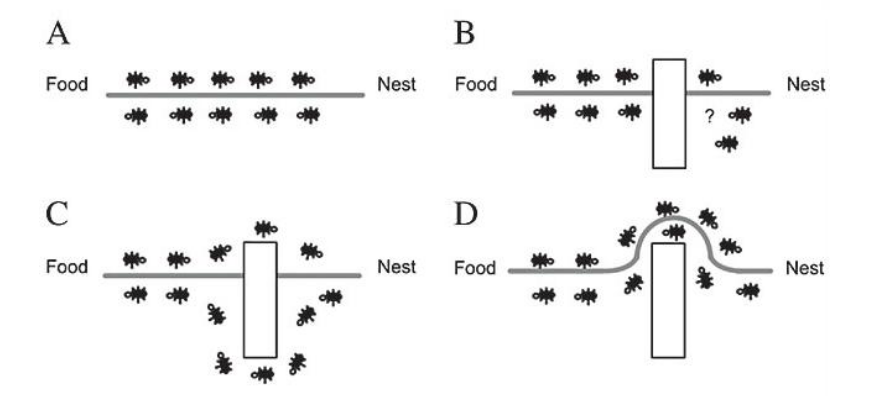
\includegraphics[width=0.7\columnwidth]{img/ants}
\end{center}
They follow the better (stronger) trail.\\

\textbf{Each agent} is an application of the basic constructive heuristic
\begin{itemize}
	\item it \textbf{leaves a trail on the data} depending on the solution generated
	
	\item it \textbf{performs choices influenced by the trails} left by the other agents
\end{itemize}

The choices of the agent have also a \textbf{random component}.\\

\newpage

\subsubsection{Trail}
As in the semi-greedy heuristic
\begin{itemize}
	\item a basic constructive heuristic $A$ is given
	\item each step performs a partially random choice
\end{itemize}

Differently from the semi-greedy heuristic
\begin{itemize}
	\item \textbf{Each iteration} $l$ \textbf{runs} $h$ \textbf{times heuristic} $A$ (population).\\
	
	\item \textbf{All} the \textbf{choices} of $\Delta_A^+ (x)$ \textbf{are feasible} (there is no RCL).\\
	
	\item The \textbf{probability} $\pi_A (i, x)$ \textbf{depends} on
	\begin{enumerate}
		\item the \textbf{selection criteria} $\varphi_A (i, x)$
		
		\item \textbf{auxiliary information} $\tau_A (i, x)$ denoted as \textbf{trail} produced in previous iterations (sometimes by other agents in the same iteration)
	\end{enumerate}
	\nn
\end{itemize}

The \textbf{trail} is \textbf{uniform at first} $(\tau_A (i, x) = \tau_0)$, and \textbf{later tuned}
\begin{itemize}
	\item \textbf{increasing} it to \textbf{favor promising choices}
	\item \textbf{decreasing} it to \textbf{avoid repetitive choices}
\end{itemize}

For the sake of simplicity, the trail $\tau_A (i, x)$ is not associated to each arc $(x, x \cup \{i\})$ (the associated data structure would be exponentially large and always way too big), but is the same for blocks of arcs (e.g., depending only on $i$, each element of the ground set).\\

\newpage

\subsubsection{Random choice}
Instead of selecting the best element according to criteria $\varphi_A (i, x)$, $i$ \textbf{is extracted from} $\Delta_A^+ (x)$ with \textbf{probability}
$$ \pi_A (i,x) = \frac{ \tau_A (i, x)^{\mu_{\tau}} \eta_A (i, x)^{\mu_{\eta} } }{ \sum_{j \in \Delta_A^+ (x)} \tau_A (j, x)^{\mu_{\tau} } \eta_A (i,x)^{\mu_{\eta} } } $$
At each step the probability is given by the values of the trail $\tau$ and the values $\eta$ related to the selection criteria.\\

where
\begin{itemize}
	\item The \textbf{denominator normalizes the probability}.\\
	
	\item The \textbf{visibility} is the \textbf{auxiliary function}
	$$ \eta_A (i,x ) =  
	\begin{cases}
		\varphi_A (i, x) & \text{ for maximization problems} \\
		\frac{1}{\varphi_A (i, x)} & \text{ for minimization problems}
	\end{cases}
	$$
	The promising choices have larger visibility.\\
	
	\item The parameters $\mu_{\tau}$ and $\mu_{\eta}$ \textbf{tune the weights} of the two terms
\end{itemize}

You are taking with larger probability elements that have a better selection criteria but that are also associated with a larger trail (they have been considered a lot in the previous iterations).\\

\newpage

\paragraph{Balancing given and learned information:} The original Ant System \textbf{tunes the probabilities with parameters} $\mu_{\eta}$ and $\mu_{\tau}$ that control the amount of randomness
\begin{itemize}
	\item $\mu_{\eta} \approx 0$ and $\mu_{\tau} \approx 0$ \textbf{push towards randomness}
	
	\item \textbf{large values} of $\mu_{\eta}$ and $\mu_{\tau}$ \textbf{push towards determinism} \\
	(favor $\arg \max_{i \in \Delta_A^+ (x)} \tau_A (i, x)^{\mu_{\tau}}  \eta_A (i, x)^{\mu_{\eta}})$
\end{itemize}

and the \textbf{relative weight of the data and of memory}
\begin{itemize}
	\item $\mu_{\eta} \gg \mu_{\tau}$ \textbf{favors the data}, simulating the basic constructive heuristic which makes sense when the known solutions are not very significant
	
	\item $\mu_{\eta} \ll \mu_{\tau}$ \textbf{favors memory}, keeping close to the previous solutions which makes sense when the known solutions are very significant
\end{itemize}

(assuming $\tau_A (i, x) > 1$ and $\eta_A (i, x) > 1$).\\

The \textbf{Ant Colony System} variant splits the selection into two phases
\begin{enumerate}
	\item \textbf{Decide the selection procedure}
	\begin{itemize}
		\item with probability $q$, to choose $i$ deterministically
		
		\item with probability $(1 − q)$, choose $i$ stochastically
	\end{itemize}
	
	where \textbf{parameter} $q$ \textbf{tunes the randomness}
	\begin{itemize}
		\item $q \approx 0$ favors random choices
		
		\item $q \approx 1$ favors deterministic choices
	\end{itemize}
	\nn
	
	\item \textbf{Apply the selection procedure}
	\begin{itemize}
		\item the \textbf{deterministic} one selects the \textbf{best element}
		$$ i^\ast = \arg \max_{i \in \Delta_A^+ (x)} \tau_A (i, x) \eta_A (i, x)^{\mu_n } $$
		
		\item the \textbf{stochastic} one select a \textbf{random element} with probabilities
		$$ \pi_A (i,x) = \frac{ \tau_A (i, x) \eta_A (i, x)^{\mu_{\eta} } }{ \sum_{j \in \Delta_A^+ (x)} \tau_A (j, x) \eta_A (i,x)^{\mu_{\eta} } } $$
	\end{itemize}
	
	where \textbf{parameter} $\mu_n$ \textbf{tunes the relative weight of data and memory}
	\begin{itemize}
		\item $\mu_n \gg 1$ favors the data
		
		\item $\mu_n \ll 1$ favors memory
	\end{itemize}
\end{enumerate}
(setting $\mu_{\tau} = 1$ as a form of normalization).\\

\newpage

\subsubsection{Trail update}
At each iteration $\ell$
\begin{enumerate}
	\item \textbf{run} $h$ \textbf{instances} of the basic heuristic $A$
	
	\item \textbf{select a subset} $\tilde{X}^{[l]}$ \textbf{of the solutions obtained}, in order to favor their elements in the following iterations
	
	\item \textbf{update the trail} according to the formula
	$$ \tau_A (i,x) := (1 - \rho) \tau_A (i,x) + \rho \sum_{y \in \tilde{X}^{[l]}: \, i \in y} F_A (y) $$
	The new trail derives from the current one with a convex combination of an additional term based off the elements of the solutions in the subset chosen and their relative fitness.
\end{enumerate}

where
\begin{itemize}
	\item $\rho \in [0; 1]$ is an \textbf{oblivion parameter} (number that reduces the current trail to give space to the new contribution)
	
	\item $F_A (y)$ is a \textbf{fitness function} expressing the \textbf{quality of solution} $y$ (such that $F > \tau :$ e.g., $F (y ) = Q/f (y )$ for a suitable constant $Q$; big if solution good, small if solution bad)
\end{itemize}

The new trail becomes a combination of the old one and a factor which scales with the quality of the solution in which a certain element is included.\\

The \textbf{purpose of the update} is to
\begin{enumerate}
	\item \textbf{increase} the \textbf{trail} on the \textbf{elements of specific solutions} ($y ∈ \tilde{X}^{[l]}$)
	
	\item \textbf{decrease} the \textbf{trail} on the \textbf{other elements}
\end{enumerate}

\newpage

\paragraph{The Oblivion parameter:} $\rho \in [0; 1]$ \textbf{tunes} the \textbf{behavior of the algorithm}:
\begin{itemize}
	\item \textbf{diversification:} a \textbf{high oblivion} ($\rho \approx 1$) \textbf{cancels the current trail} based on the intuition that
	\begin{itemize}
		\item the solutions obtained are not trustworthy
		\item different solutions should be explored
	\end{itemize}
	
	\item \textbf{intensification:} a \textbf{low oblivion} ($\rho \approx 0$) \textbf{preserves the current trail} based on the intuition that
	\begin{itemize}
		\item the solutions obtained are trustworthy
		\item similar solutions should be explored
	\end{itemize}
\end{itemize}
\nn

\paragraph{Selection of the influential solutions:} $\tilde{X}^{[l]}$ collects the \textbf{solutions around which the search will be intensified}
\begin{itemize}
	\item the classical Ant System considers all the solutions of iteration $l - 1$
	
	\item the \textbf{elitist methods} consider the best known solutions
	\begin{itemize}
		\item the best solution of iteration $l - 1$
		\item the best solution of all iterations $< l$
	\end{itemize}
	You look for an "elite" solution, the best solution in respect to something (all iterations/this iteration)
\end{itemize}

The elitist methods
\begin{itemize}
	\item find \textbf{better results in shorter time}
	
	\item require \textbf{additional mechanisms} to \textbf{avoid premature convergence}
\end{itemize}
\nn

\newpage

\paragraph{Some variants of the Ant System:}
\begin{itemize}
	\item \textbf{MAX $-$ MIN Ant System:} imposes on the trail a limited range of values $[\tau_{min}; \tau_{max}]$, experimentally tuned.\\
	
	\item \textbf{HyperCube Ant Colony Optimization (HC-ACO):} normalizes the trail between 0 and 1.\\
	
	\item Ant Colony System: updates the trail on two levels
	\begin{itemize}
		\item the \textbf{global update} (already seen) modifies it at each iteration $\ell$ (the purpose is to intensify the search)
		
		\item the \textbf{local update} updates the trail at each application $g$ of the basic heuristic in order to discourage identical choices in the following
		$$ \tau_A (i, x) := (1 - \rho) \tau_A (i, x) \text{ for each } i \in x^{[l,g]}$$
	\end{itemize}
	\nn
\end{itemize}
The purpose is to diversify the search.\\

\newpage

\subsubsection{Convergence to the optimum}
\textbf{Some variants} of the Ant System \textbf{converge to the optimum} with probability $1$ (Gutjahr, 2002).\\

The \textbf{analysis} is \textbf{based on the construction graph}
\begin{itemize}
	\item The \textbf{trail} $\tau_A (i, x)$ is laid down \textbf{on the arcs} $(x, x \cup \{i\})$.\\
	
	\item \textbf{No information from the data} is used, that is $\eta_A (i, x) \equiv 1$ (only the trail, no data; this strange assumption simplifies the computation, but is not necessary).\\
	
	\item $\tau^{[l]}$ is the \textbf{trail function} at the \textbf{beginning of iteration} $l$.\\
	
	\item $\gamma^{[l]}$ is the \textbf{best path} on the graph at the \textbf{end of iteration} $l$.\\
	
	\item $(\tau^{[l]}, \gamma^{[l−1]})$ is the \textbf{state of a non-homogeneous Markov process}:
	\begin{itemize}
		\item the \textbf{probability of each state} depends only on the \textbf{previous iteration}
		
		\item the \textbf{process} is \textbf{non-homogeneous} because the \textbf{dependency varies with} $l$
	\end{itemize}
\end{itemize}

The \textbf{proof concludes} that for $\ell \rightarrow + \infty$, with probability $1$
\begin{enumerate}
	\item the \textbf{best path found} $\gamma$ \textbf{is one of the optimal paths} in $\mathcal{F}$
	
	\item the \textbf{trail} $\tau$ \textbf{tends to a maximum along} $\gamma$, to zero on the other arcs
\end{enumerate}
provided that a suitable parameter tuning is adopted.\\

\newpage

\paragraph{First variant with global convergence:} The \textbf{trail} is \textbf{updated} with a \textbf{variable coefficient of oblivion}
$$ \tau^{[l]} (i, x) := 
\begin{cases}
	(1  -\rho)^{[l-1]} \tau^{[l-1]} (i,x) + \rho^{[l-1]} \frac{1}{|\gamma^{[l-1]}|} & \text{ if } (x, x \cup \left\{i\right\}) \in \gamma^{[l-1]} \\
	(1  -\rho)^{[l-1]} \tau^{[l-1]} (i,x) & \text{ otherwise }
\end{cases}
$$
where $\gamma^{[l−1]}$ is the \textbf{best path found} in the graph \textbf{up to iteration} $l - 1$ and $|\gamma^{[l−1]}|$ is the \textbf{number of its arcs} (to normalize the trail).\\

The idea is that if you're considering the best known path up until that point ($(x, x \cup \left\{i\right\}) \in \gamma^{[l-1]}$, elitist strategy) then you are going to increase the trail on that path by a certain amount (1 divided by the number of arcs on that path). If an arc is not on the best known path you just decrease the trail.\\

Differences: the objective function is not considered since data is not taken into account, and the oblivion parameter is not fixed (decreases, but not very fast).\\

\textbf{If the oblivion decreases slowly enough}
$$ \rho^{[l]} \leq 1 - \frac{\log l}{\log (l+1)} \;\;\; \text{ and } \;\;\; \sum_{l=0}^{+ \infty} \rho^{[l]} = + \infty $$
First half puts a bound to the value of the parameter, which will be forced to decrease. The second part means that the sum of all parameters should diverge, i.e. it should not decrease too fast (otherwise there's the risk of a premature convergence).\\

Then with probability $1$ \textbf{the state converges to} $(\tau^\ast, \gamma^\ast)$, where
\begin{itemize}
	\item $\gamma^\ast$ \textbf{is an optimal path} in the construction graph
	
	\item $\tau^\ast (i, x) = 1/|\gamma^\ast|$ for $(x, x \cup \{i\}) \in \gamma^\ast$, $0$ otherwise
\end{itemize}

\newpage

\paragraph{Second variant with global convergence:} Alternatively, if the \textbf{oblivion} $\rho$ \textbf{remains constant}, but the \textbf{trail is forced a slowly decreasing minimum threshold}
$$ \tau (i,x) \geq \frac{c_l}{\log(l+1)} \text{ and } \lim_{l \rightarrow + \infty} c_l \in (0;1)$$
then with probability $1$ \textbf{the state converges to} $(\tau^\ast, \gamma^\ast)$.\\

Here the oblivion is restricted by the minimum threshold.\\

The trail must always be larger than the first term and it means that the trail must not decrease to zero too fast, otherwise there could be a premature convergence, but its limit must be finite, so it must not be too slow.\\ 


\textbf{In practice}, all algorithms proposed so far in the literature
\begin{itemize}
	\item associate the trail to groups of arcs $(x, x \cup \{i\})$ (e.g., to each element $i$)
	
	\item use constant values for parameters $\rho$ and $\tau_{min}$
\end{itemize}
therefore do not guarantee convergence.\\

The trail $\tau$, and therefore $\pi$, can tend to zero on every optimal path.\\

% End of L11, L12 is a lab, so next is L13

\newpage